\documentclass[10pt,handout]{beamer}

\usepackage[french]{babel}
\usepackage[T1]{fontenc}
\usepackage[utf8]{inputenc}
\usepackage[
    left = \flqq{},%
    right = \frqq{},%
    leftsub = \flq{},%
    rightsub = \frq{} %
]{dirtytalk} 	% for \say{}
\usepackage{xcolor} 	% for color text
\usepackage{csquotes}
\usepackage{amssymb}
\usepackage{mathtools}
\usepackage{array}

\usetheme{Frankfurt}
\usetheme{CambridgeUS}
\usetheme{JuanLesPins}
%\usetheme{Montpellier}
%\usetheme{Madrid}

\usecolortheme{dolphin}

\useinnertheme{circles}
\usefonttheme{structurebold}
\useoutertheme{default}

%\hypersetup{pdfpagemode=FullScreen}

\title[Mini-Projet Entrepôt de données]{Air France}
\author[Bouzidi, Elhouiti, Kezzoul]{Bouzidi Belkacem - Elhouiti Chakib \\ Kezzoul Massili}
\institute[]{Université de Montpellier}
\date{\today}


% Mettre les listes en triangle
\setbeamertemplate{itemize item}[triangle]

%Insertion d'un logo
\newif\ifplacelogo % create a new conditional
\placelogotrue % set it to true
\logo{\ifplacelogo
\includegraphics[height=12mm]{img/univ-montpellier.png}\fi}

%------------------------------------------------------%
% page de titre
%------------------------------------------------------%
\begin{document}

\placelogofalse
\begin{frame}
	\titlepage
\end{frame}

\placelogotrue


%------------------------------------------------------%
% Intro
%------------------------------------------------------%
\section{Introduction}
\placelogofalse
\begin{frame}{Présentation de l'entreprise}{AirFrance}
  \begin{block}{Objectifs}
    Le premier objectif d’Air Fance est de développer son réseau, de développer ses possibilités de destinations tout en réduisant les coûts. Au même temps assurer une prestation de service de haute qualitée.
  \end{block}

  \begin{block}{Position sur le marché}
    Air France est l’une des leader du transport aérien européen.
  \end{block}

\end{frame}

\begin{frame}{Analyse du cas}
  \begin{block}{Identification des informations à tracer}
    \begin{itemize}
     \item la date de la vente.
     \item le lieux de depart et d’arrivé(distination en vogue).
     \item le prix de vente du billet.
     \item Nombre de place occupé dans l’avion.
     \item rentabilité du vol (revenu/dépenses)
     \item La tranche de chaque client.
     \item La fidelité de chaque client.
     \item Nombre de billets enregistrés pour chaque client
     \item position de chaque avion à la fin de la journée (aéroports)
     \item consommation d’un avion (carburant et divers coûts)
     \item nombre de vol effectués par un avion.
    \end{itemize}
  \end{block}
\end{frame}

%------------------------------------------------------%
% Modélisation
%------------------------------------------------------%

\section{Modélisation}

\begin{frame}{Ventes des billets}
  \begin{figure}
    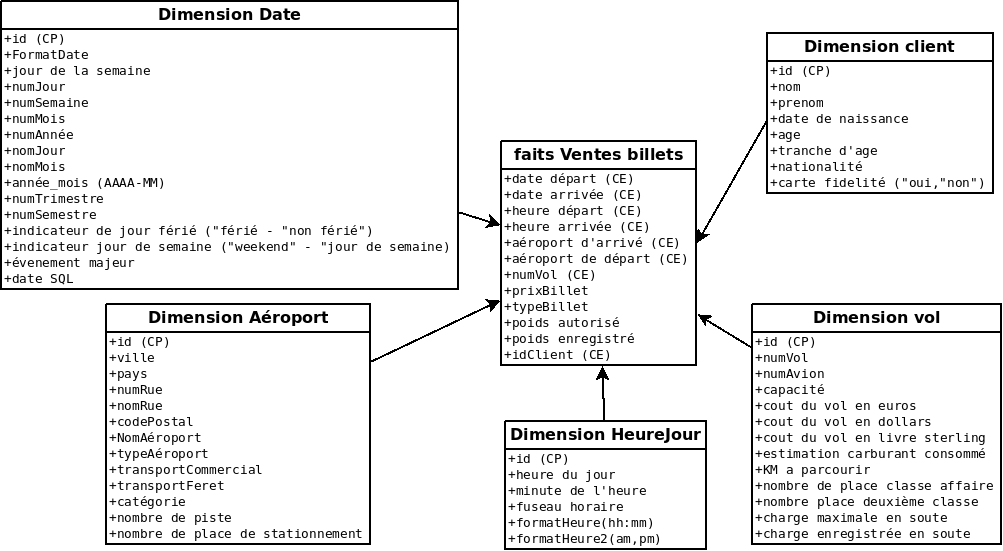
\includegraphics[width=12cm]{img/VenteBillet.png}
  \end{figure}
\end{frame}

\begin{frame}{Stock d'avions}
  \begin{figure}
    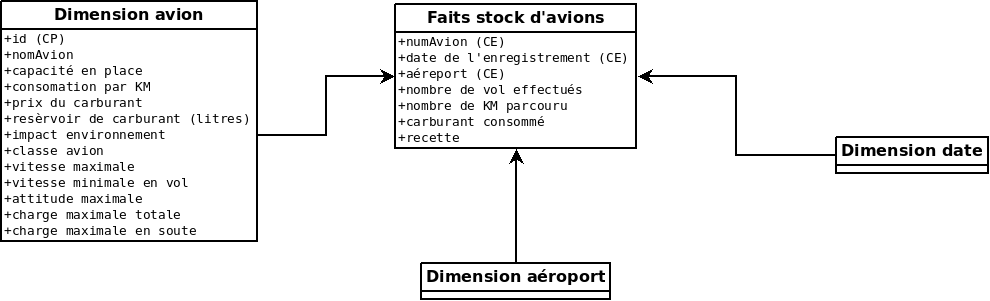
\includegraphics[width=12cm]{img/flotteAvions.png}
  \end{figure}
\end{frame}

%------------------------------------------------------%
% Implémentation
%------------------------------------------------------%
\section{Requêtage}
\begin{frame}{Requêtes analytiques}
  blabla
\end{frame}

\section{Estimation de la taille de l'entrepôt}
\begin{frame}{Estimation de la taille de l'entrepôt}
  \begin{figure}
    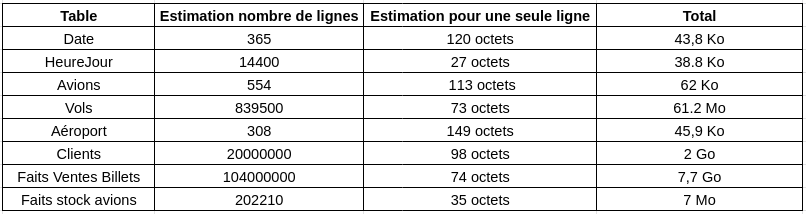
\includegraphics[width=12cm]{img/estimation_taille.png}
  \end{figure}
\end{frame}

\section{Implémentation}

\begin{frame}{Implémentation des Data-Mart}
  \begin{block}{Création des tables}
    Création des tables de dimension en premier, ensuite la création des tables de faits.
  \end{block}
  \begin{block}{Vues}
    Utilisage des vues pour faciliter une reqûete analytique qui utilise le résultat d'une autre reqûete (un calcul).
  \end{block}
\end{frame}


\end{document}
